\section*{Comunicazioni analogiche}

Amplitude Modulation Dual Side Band (AM-DSB) è generalmente utilizzata per trasmettere solo la voce. 


Il segnale \( s_{DSB}(t) \) è definito come:

\begin{equation*}
s_{DSB}(t) = A_c m(t) \cos(2\pi f_c t)
\end{equation*}

\begin{center}
    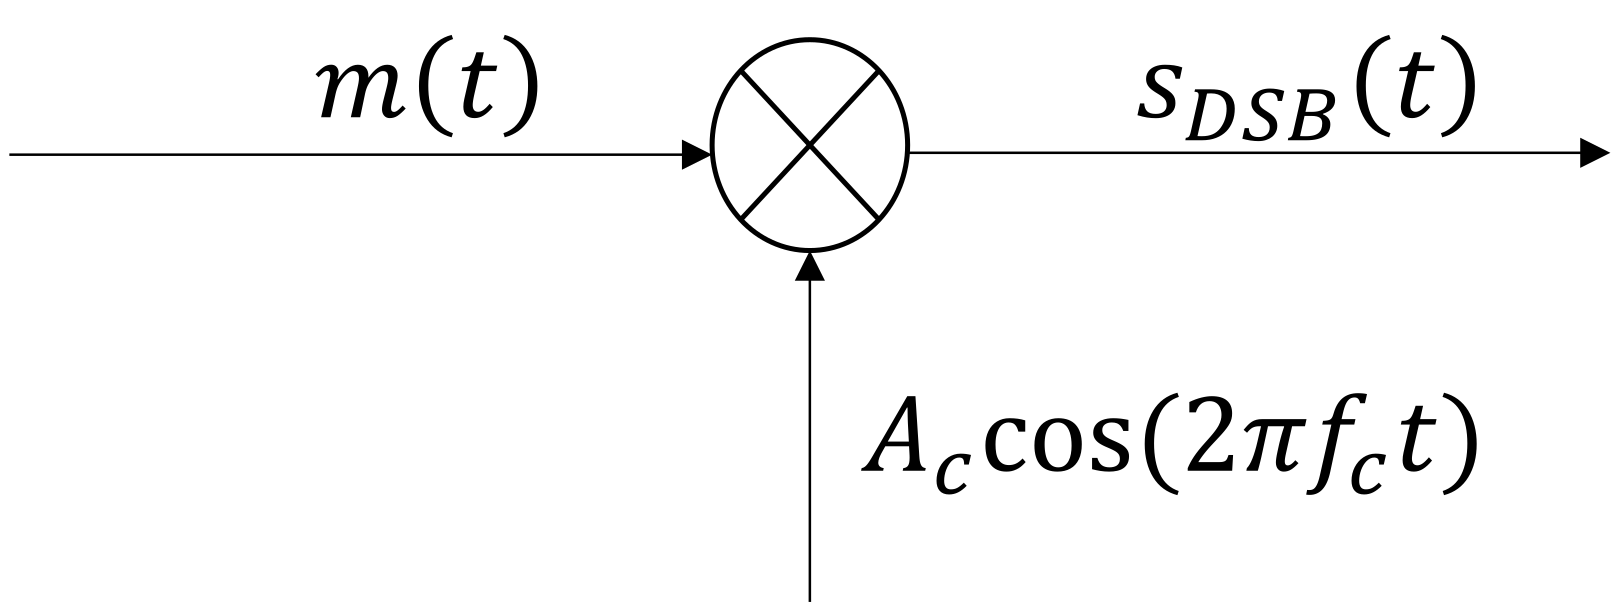
\includegraphics[width=0.25\textwidth]{imgs/analog_pam_trasmitter.png}
\end{center}


dove:
\begin{itemize}
    \item \( m(t) \) è il segnale modulante o il messaggio.
    \item \( A_c \) è l'ampiezza del segnale portante.
    \item \( \cos(2\pi f_c t) \) è l'onda portante alla frequenza \( f_c \).
\end{itemize}

\begin{center}
    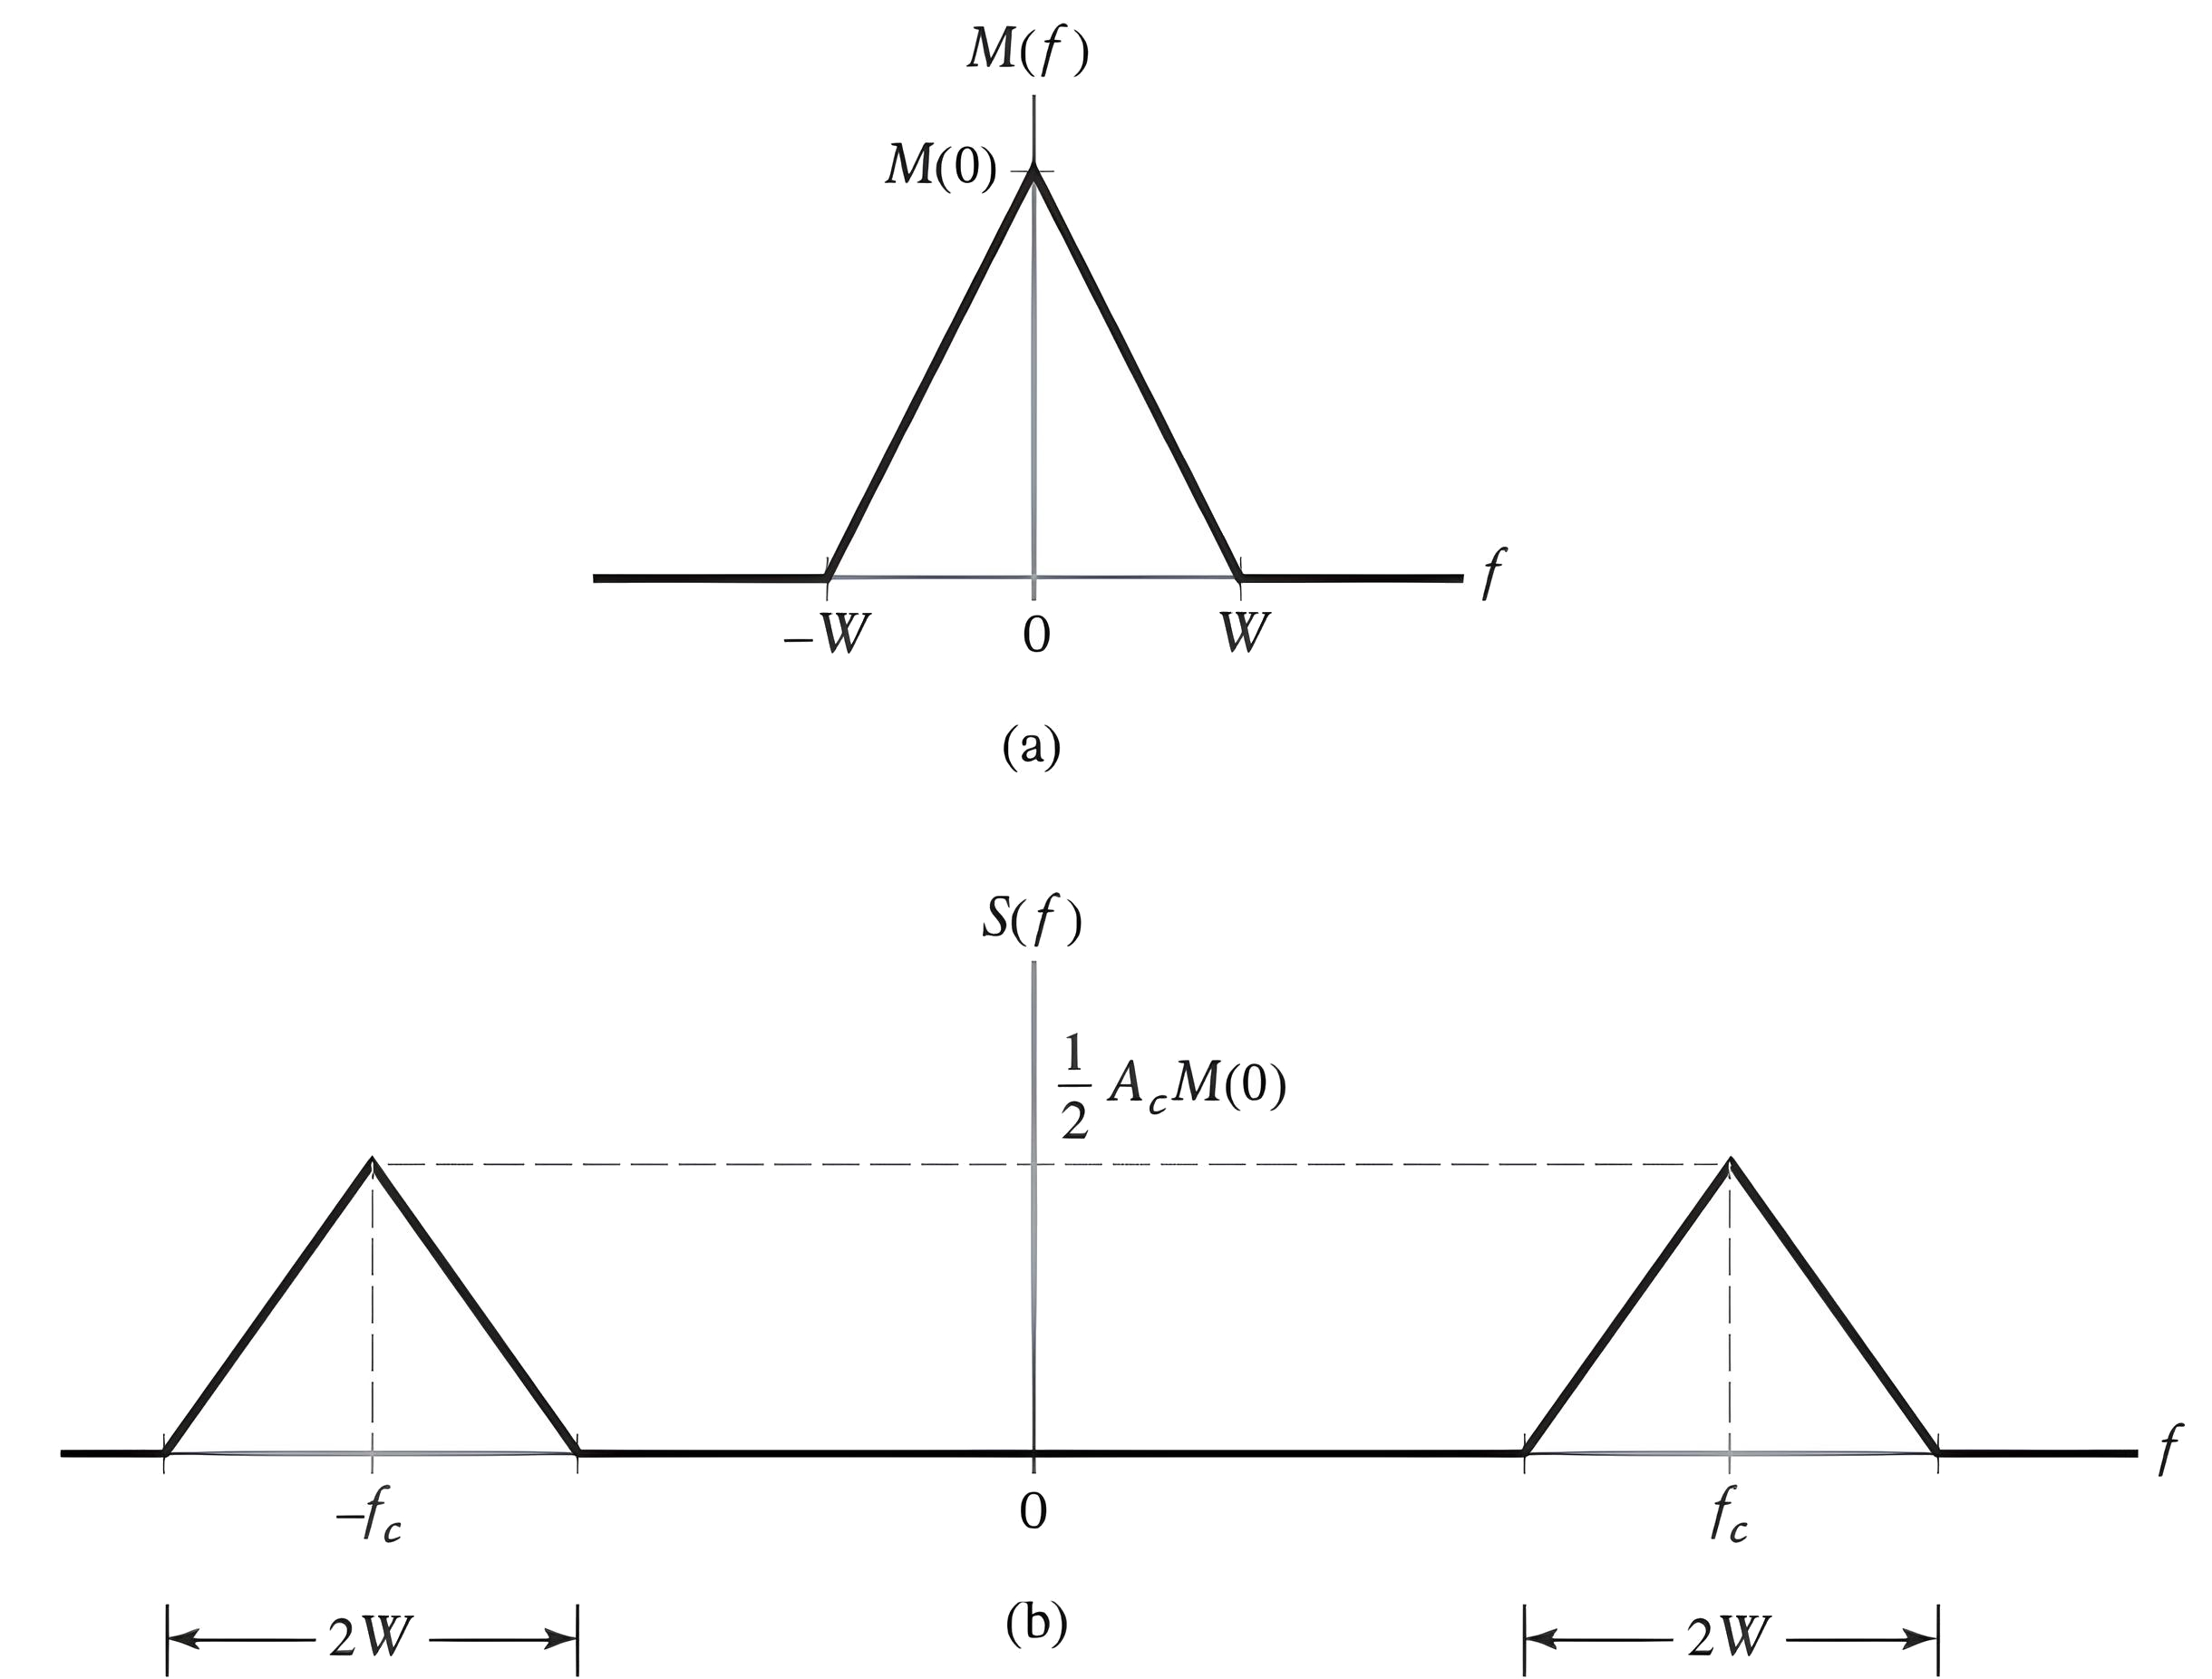
\includegraphics[width=0.5\textwidth]{imgs/dsb.jpg}
\end{center}


La modulazione AM-DSB è caratterizzata da due sideband, ciascuno localizzato tra \( f_c \pm W \) e \( -f_c \pm W \), dove \( W \) è la banda del segnale modulante. Questi sideband trasportano la stessa informazione, da cui il termine \textbf{dual sideband}.

Effettuando la trasformata di Fourier\footnote{$X(f) \triangleq \int_{-\infty}^{+\infty} x(t) e^{-j2\pi ft} dt$} di \( s_{DSB}(t) \), otteniamo la rappresentazione nel dominio delle frequenze \( S_{DSB}(f) \). Ciò è calcolabile come segue:
\[  
    S_{DSB}(f) = A_c \ \mathcal{F}\{m(t)\} (f)  \ast \mathcal{F}\{\cos(2\pi f_c t) \}(f) = A_c M(f) \ast \frac{\delta(f - f_c) + \delta(f + f_c)}{2} =
\]

\[
= \frac{1}{2} A_c [M(f - f_c) + M(f + f_c)]
\]
Sebbene la componente negativa possa essere trascurata adesso la traslazione del segnale alla frequenza $f_c \gg W$ comporta un'occupazione di banda di $2W$ per ogni lato, ma ciò comporta uno spreco in quanto si ha duplicazione di informazione. 

\begin{center}
    \begin{tikzpicture}
    \begin{axis}[
        title={AM-DSB Modulation},
        xlabel={Time},
        ylabel={Amplitude},
        axis lines=middle,
        ymax=2,
        ymin=-2,
        xtick=\empty,
        ytick=\empty,
        clip=false,
        no markers,
        width=10cm,
        height=5cm
    ]
    \addplot [domain=0:2*pi, samples=100, name path=m] {sin(deg(x))};
    \addlegendentry{$m(t)$}

    \addplot [domain=0:2*pi, samples=100, name path=carrier] {1.5*cos(deg(5*x))};
    \addlegendentry{$A_c \cos(2\pi f_c t)$}

    \addplot [domain=0:2*pi, samples=100, red, name path=am] {1.5*sin(deg(x))*cos(deg(5*x))};
    \addlegendentry{$s_{DSB}(t)$}

    \addplot [domain=0:2*pi, samples=100, dashed, name path=upper] {1.5*sin(deg(x))};
    \addplot [domain=0:2*pi, samples=100, dashed, name path=lower] {-1.5*sin(deg(x))};

    \addplot[fill=gray!30] fill between[of=upper and lower];

    \end{axis}
    \end{tikzpicture}
\end{center}


Il segnale \( s_{DSB}(t) \) dopo essere stato filtrato dal filtro passa-banda (BPF) conserva la sua forma.
La rilevazione coerente è implementata moltiplicando \( s_{DSB}(t) \) con una portante sincronizzata \( 2\cos(2\pi f_c t) \).
Questo comporta la presenza di una componente ad alta frequenza a \( 2f_c \) che viene rimossa dal filtro passa-basso (LPF), lasciando solo il segnale messaggio \( m(t) \).
\begin{center}
    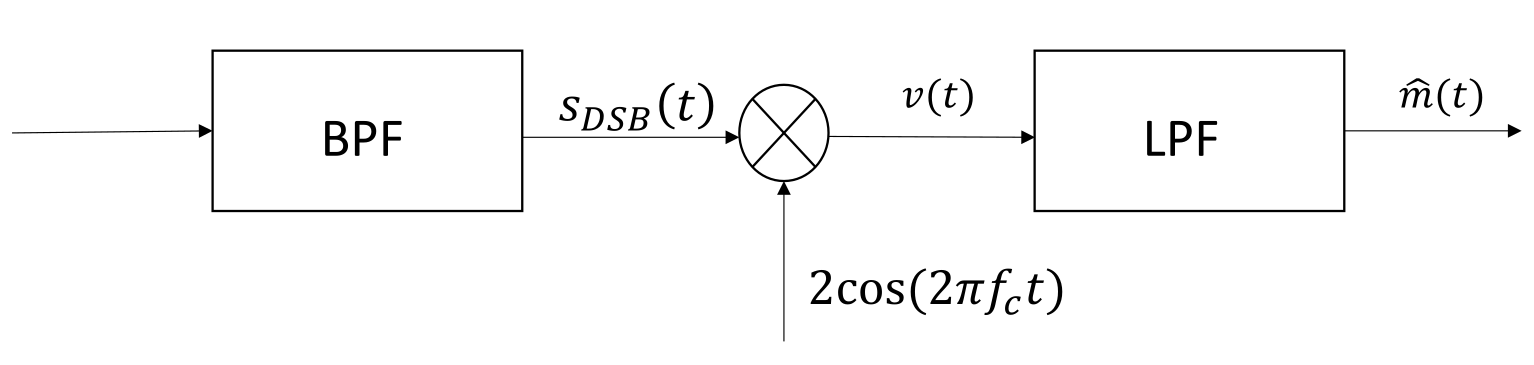
\includegraphics[width=0.625\textwidth]{imgs/analog_pam_receiver.png}
\end{center}

Dopo la demodulazione e il filtraggio, lo spettro è centrato nuovamente in banda base, recuperando il segnale messaggio.

Possiamo definire $B = f_c + W$ come la banda di trasmissione se consideriamo il massimo o $B = 2W$ se consideriamo quanto occupa.
Nella radio AM si ha una carrier frequency tra i 500 e i 1600 kHz e una $W$ tra i 5 e i 10 kHz.
Il segnale è pari (in modulo) a causa della simmetria hermitiana, infatti essendo $m(t)$ reale, $M(-f) = M^*(f)$ e quindi $|M(-f)| = |M(f)|$.


La ricostruzione del segnale originario richiede tre step:
\begin{itemize}
  \item \textbf{Filtraggio passa-banda}: il segnale ricevuto è filtrato tramite un filtro passa-banda, centrato in \( f_c \), per rimuovere le componenti fuori banda.
  \item \textbf{Demodulazione}: il segnale modulato viene moltiplicato per un secondo coseno, ottenendo oltre al segnale originario anche due contributi in \(\pm 2f_c \)
  \item \textbf{Filtraggio passa-basso}: il segnale demodulato viene filtrato con un filtro passa basso di ampiezza W, per rimuovere la componente ad alta frequenza.
\end{itemize}

\begin{equation*}
    v(t) = s_{DSB}(t) \cdot 2\cos(2\pi f_c t) = A_c m(t) \cdot 2\cos^2(2\pi f_c t) = A_c m(t) + A_c m(t) \cos(4\pi f_c t)
\end{equation*}

L'ipotesi $f_c^{(t)} = f_c^{(r)}$ garantisce la possibilità di effettuare il passaggio trigonometrico e dunque riscostruire il segnale originario senza alcuna distorsione. Tuttavia a prescindere dalla bontà dell'oscillatore utilizzato non è possibile ottenere una sincronizzazione perfetta senza alcuna logica aggiuntiva, un reale sistema di modulazione AM prevede tale meccanismo.

\section*{Analog Quadrature Amplitude Modulation}

\begin{center}
    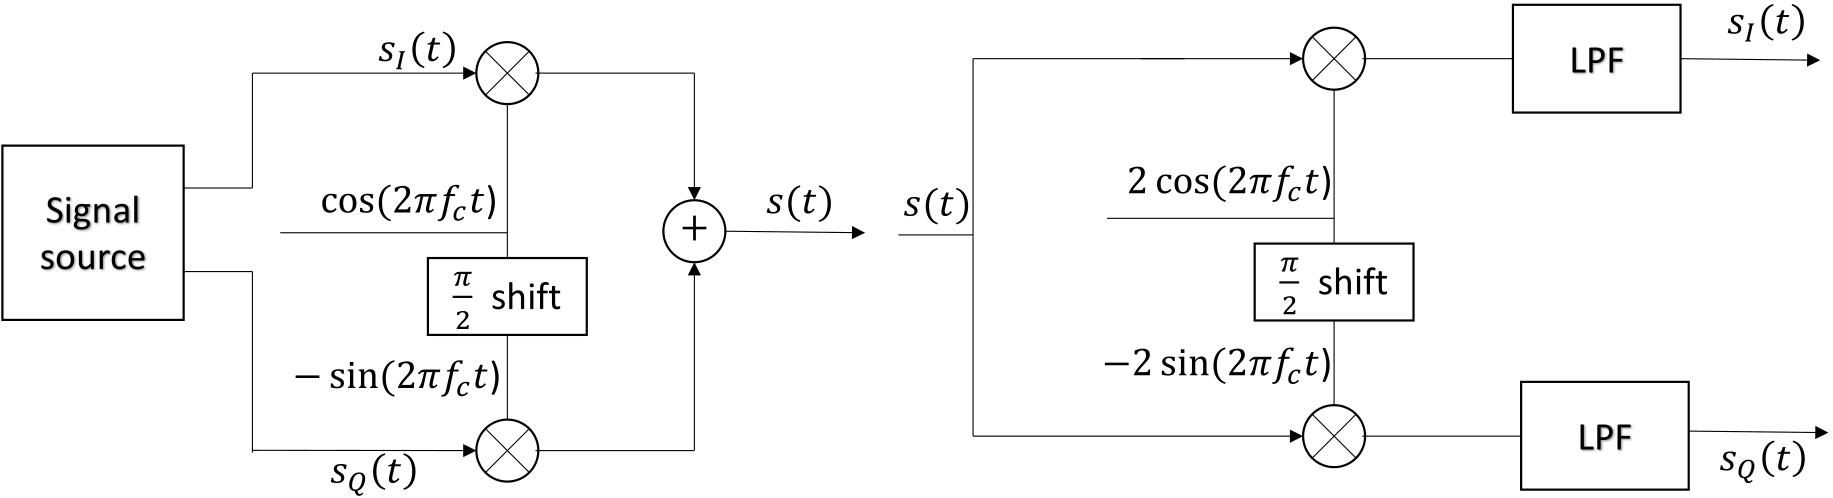
\includegraphics[width=1\textwidth]{imgs/analog_qam.png}
\end{center}

















Per raddoppiare la quantità di informazioni trasmesse all'interno della stessa banda si può sfruttare l'ortogonalità della funzione seno e coseno, in modo da trasmettere contemporaneamente due segnali, occupando in modo ottimale la banda a disposizione. Tale modulazione è detta QAM, il termine quadrature indica lo shift di $\pi/2$ tra le due funzioni portant (seno e coseno), mentre amplitude ricorda che si tratta comunique di una modulazione in cui l'informazione è trasportata interamente dall'ampiezza del segnale. L'ampiezza del segnale portante è infatti modulata in modo proporzionale all'ampiezza del segnale modulante, contente l'informazione da trasmettere.





Il segnale composto QAM \( s(t) \) può essere rappresentato come la somma di due segnali modulati DSB, uno modulato con un coseno (la componente in fase) e l'altro con un seno (la componente in quadratura):
\begin{equation}
s_{QAM}(t) = A_{c} m_1(t) \cos(2\pi f_c t) - A_{c} m_2(t) \sin(2\pi f_c t)
\end{equation}

Dove:
\begin{itemize}
    \item \( m_1(t) \) e \( m_2(t) \) sono i segnali che contengono il messaggio per le componenti in fase e in quadratura, rispettivamente.
    \item \( f_c \) è la frequenza della portante.
\end{itemize}


La demodulazione del segnale QAM è effettuata moltiplicando il segnale composto \( s(t) \) con \( 2\cos(2\pi f_c t) \) e \( -2\sin(2\pi f_c t) \) per ottenere le componenti in fase \( s_I(t) \) e in quadratura \( s_Q(t) \), rispettivamente.
Questi prodotti sono poi filtrati con filtri passa-basso per estrarre i segnali contenenti il messaggio originali \( m_1(t) \) e \( m_2(t) \).
La demodulazione è fatta nella seguente maniera:
\begin{equation}
    v_I(t) = s(t) \cdot 2\cos(2\pi f_c t) = A_{c} m_1(t) + A_{c} m_1(t) \cos(4\pi f_c t) - A_{c} m_2(t) \sin(4\pi f_c t)
\end{equation}
\begin{equation}
    v_Q(t) = s(t) \cdot (-2\sin(2\pi f_c t)) = A_{c} m_2(t) - A_{c} m_1(t) \cos(4\pi f_c t) - A_{c} m_2(t) \sin(4\pi f_c t)
\end{equation}

Le componenti ad alta frequenza sono filtrate dal filtro passa-basso, ottenendo così i segnali originali \( m_1(t) \) e \( m_2(t) \).
Lo spettro del segnale ottenuto tramite moduazione non risulta più simmetrico rispetto a $f_c$, tuttavia essendo un segnale reale resta valida la simmetria rispetto all'asse delle ordinate.
La mancanza di simmetria rispetto a $f_c$ implica la non esistenza di un segnale reale in grado di rappresentare lo spettro in banda base, in quanto verrebbe meno la simmetria rispetto alla frequenza 0.
Sebbene questa mancanza non precluda l'utilizzo della modulazione QAM, nella pratica risulta più semplice lo studio di un segnale in banda base.
\begin{itemize}
    \item La carrier frequency \( f_c \) non aggiunge informazione al segnale, ma viene utilizzata per traslare il segnale in frequenza.
    \item Il criterio di Nyquist richiede un compionamento ad una frequnza doppia rispetto alla banda del segnale, quindi nel caso di segnale passa-banda tale valore può essere molto elevato. Nel caso di segnale in banda base la frequenza di campionamento può essere nettamente inferiore.
\end{itemize}

Il criterio di Nyquist stabilisce che \( T \leq \frac{1}{2B} \), dove \( T \) è il periodo di campionamento e \( B \) è la banda del segnale, e quindi \( f_s \geq 2B \). Quindi nel nostro caso, $f_s \geq 2(f_c + W)$.
Un segnale è definito in passa banda quando la propria energia è concentrata all'interno di una banda $2W$ centrata attorno a una carrier frequency $f_c$, con il vincolo $f_c \gg W$.  

\subsection*{Inviluppo Complesso di un Segnale in Banda Passante}
\begin{center}
    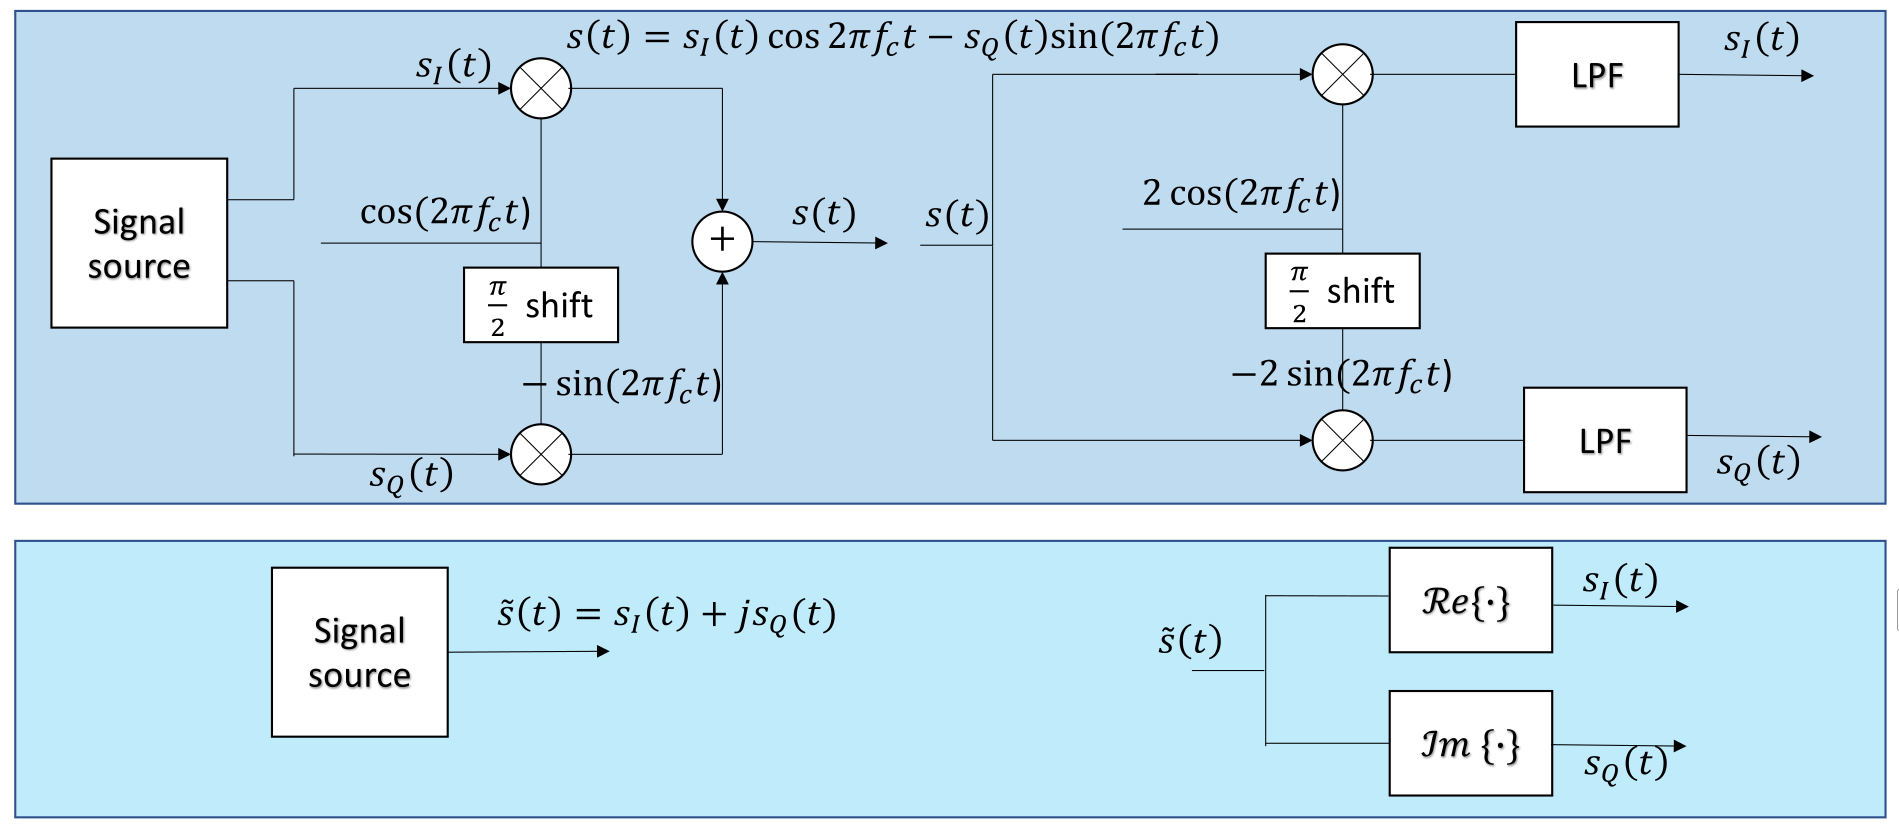
\includegraphics[width=1\textwidth]{imgs/complex_envelope.png}
\end{center}
La maggior parte dei sistemi di comunicazione opera in banda passante. Il segnale trasmesso \( s(t) \), concentrato in una banda di frequenza \( 2B \) e centrato attorno a una frequenza portante \( f_c \), risiede ben al di sopra della corrente continua (DC) o frequenza zero. Per un segnale in banda passante, vale la condizione \( f_c \gg 2B \), indicando che la frequenza portante è molto maggiore del doppio della larghezza di banda del segnale.

L'assenza di un segnale in banda base ha portato all'adozione dell'inviluppo complesso, definito come:
\begin{equation}
    \tilde{s}(t) = s_I(t) + js_Q(t) = A(t)e^{j\phi(t)}
\end{equation}
\begin{equation}
    s(t) = \Re\{\tilde{s}(t)e^{j2\pi f_c t}\} = s_I(t)\cos(2\pi f_c t) - s_Q(t)\sin(2\pi f_c t)
\end{equation}

Questo inviluppo complesso permette di rappresentare \( s(t) \) come la parte reale del prodotto del suo inviluppo complesso per un esponenziale complesso alla frequenza portante, facilitando l'analisi e la modulazione del segnale nei sistemi di comunicazione digitale. Per esempio, nella modulazione AM si ottiene:
\begin{equation}
    \tilde{s}_{AM}(t) = m(t) = A(t)e^{j\phi(t)}
\end{equation}
dove \( \phi(t) \) assume valore \( 0 \) o \( \pi \), essendo assente la componente immaginaria.

La sincronizzazione del clock tra trasmettitore e ricevitore è cruciale per una ricostruzione perfetta dell'informazione trasmessa, mantenendo la caratteristica di ortogonalità perfetta tra seno e coseno, necessaria per separare i due messaggi una volta modulati.

L'inviluppo complesso rappresenta un modello equivalente in banda base che facilita l'analisi e l'elaborazione dei segnali in banda passante come se fossero segnali in banda base, offrendo numerosi vantaggi:
\begin{itemize}
    \item Il modello in banda base è più semplice da studiare, poiché elimina gli effetti della frequenza portante dal modello del segnale, semplificando l'analisi matematica e la comprensione delle proprietà del segnale.
    \item La simulazione numerica di un modello in banda base richiede meno risorse computazionali rispetto a un modello in banda passante, grazie alla minor larghezza di banda necessaria.
    \item Di conseguenza, anche la frequenza di campionamento è inferiore per i modelli in banda base, il che si traduce in tassi di trasmissione dati ridotti, vantaggioso per l'elaborazione e lo stoccaggio del segnale digitale.
    \item Il modello in banda base è spesso la base per un'implementazione digitale di un sistema di comunicazione in banda passante, facilitando l'applicazione delle tecniche di elaborazione del segnale digitale, fondamentali nelle comunicazioni moderne.
\end{itemize}

\section*{Modulazione di Frequenza (FM)}

Nella modulazione di frequenza (FM), il messaggio è incorporato nella fase del segnale \( \phi(t) \). Il segnale FM \( s_{FM}(t) \) può essere espresso come:
\begin{equation}
    s_{FM}(t) = A_c \cos\left(2\pi f_c t + 2\pi k_f \int_{-\infty}^{t} m(\tau) d\tau \right)
\end{equation}

La fase \( \phi(t) \) del segnale FM è quindi data dall'integrale del segnale del messaggio \( m(t) \), scalato dalla sensibilità alla deviazione di frequenza \( k_f \):
\begin{equation}
    \phi(t) = 2\pi f_c t + 2\pi k_f \int_{-\infty}^{t} m(\tau) d\tau
\end{equation}

L'indice di modulazione \( m_f \) è definito come il rapporto tra la deviazione di frequenza e la larghezza di banda del messaggio \( B_m \):
\begin{equation}
    m_f = \frac{\Delta f}{B_m}
\end{equation}

%Δ𝑓 = max |𝑓7 (𝑡)| = 𝑘) max 𝑚(𝑡)
Dove $\Delta f = \max |f(t)| = k_f \max m(t)$.
La rappresentazione complessa del segnale FM può essere ottenuta utilizzando la formula di Eulero:
\begin{equation}
    s_{FM}(t) = \Re \left\{ A_c e^{j\phi(t)} \right\} = \Re \left\{ A_c e^{j2\pi f_c t} e^{j2\pi k_f \int_{-\infty}^{t} m(\tau) d\tau} \right\} = \Re \left\{ \tilde{s}_{FM} (t) e^{j2\pi f_c t} \right\}
\end{equation}

E quindi:
\begin{equation}
    \tilde{s}_{FM}(t) = A_c e^{j2\pi k_f \int_{-\infty}^{t} m(\tau) d\tau}
\end{equation}

Questa rappresentazione è particolarmente utile per l'analisi dei segnali FM nel contesto del trattamento digitale dei segnali.

I vantaggi della modulazione in frequenza includono:
\begin{itemize}
    \item Minore sensibilità ai disturbi, migliorando così la qualità del segnale ricevuto.
    \item Maggiore efficienza energetica, poiché il segnale informativo non richiede potenza aggiuntiva a quella della portante.
    \item L'ampliezza costante permette l'uso di amplificatori semplificati in fase di trasmissione, evitando la necessità di mantenere l'amplificatore nella zona lineare, come sarebbe necessario con le modulazioni di ampiezza variabile (AM).
    \item Possibilità di configurare la modulazione per ottimizzare il compromesso tra qualità della trasmissione e banda occupata.
\end{itemize}



\begin{center}
    \resizebox{0.5\textwidth}{!}{
        \begin{tikzpicture}[align=center]
            \begin{groupplot}[
                group style={
                    group size=1 by 3,
                    vertical sep=1cm
                },
                width=14cm,
                height=5cm
            ]
           
            \nextgroupplot[
                xmin=0, xmax=12,
                ymin=-1.5, ymax=1.5,
                axis lines=middle,
                xtick=\empty,
                ytick=\empty,
                xlabel={},
                ylabel={},
                title={Carrier ($f_c$)} 
            ]
            \addplot[thick, domain=0:12, samples=200] {sin(deg(2*3.14*x))};
            \nextgroupplot[
                xmin=0, xmax=12,
                ymin=-1.5, ymax=1.5,
                axis lines=middle,
                xtick=\empty,
                ytick=\empty,
                xlabel={},
                ylabel={},
                title={Baseband Input ($f_m$)}
            ]
            \addplot[thick, domain=0:12, samples=200] {sin(deg(0.3*3.14*(x - 1.57)))};
           
            \draw[dashed] (axis cs:1.57,25) -- (axis cs:1.57,-25);
            \draw[dashed] (axis cs:3.235,25) -- (axis cs:3.235,-25);
            \draw[dashed] (axis cs:4.9,25) -- (axis cs:4.9,-25);
            \draw[dashed] (axis cs:6.565,25) -- (axis cs:6.565,-25);
            \draw[dashed] (axis cs:8.23,25) -- (axis cs:8.23,-25);
            \draw[dashed] (axis cs:9.895,25) -- (axis cs:9.895,-25);
            \draw[dashed] (axis cs:11.56,25) -- (axis cs:11.56,-25);
        
            \nextgroupplot[
                xmin=0, xmax=12,
                ymin=-2, ymax=1.5,
                axis lines=middle,
                xtick=\empty,
                ytick=\empty,
                xlabel={},
                ylabel={},
                title={FM waveform}
            ]
            \addplot[thick, domain=0:12, samples=200] {sin(deg(2*3.14*(x-0.5*sin(deg(0.3*3.14*(x))))))};
            \draw[dashed] (axis cs:1.57,25) -- (axis cs:1.57,-25);
            \draw[dashed] (axis cs:3.235,25) -- (axis cs:3.235,-25);
            \draw[dashed] (axis cs:4.9,25) -- (axis cs:4.9,-25);
            \draw[dashed] (axis cs:6.565,25) -- (axis cs:6.565,-25);
            \draw[dashed] (axis cs:8.23,25) -- (axis cs:8.23,-25);
            \draw[dashed] (axis cs:9.895,25) -- (axis cs:9.895,-25);
            \draw[dashed] (axis cs:11.56,25) -- (axis cs:11.56,-25);
        
            \draw[->, thick] (axis cs:0.1,-1.4) -- (axis cs:1.47,-1.4) node[midway, below] {f. increase};
            \draw[->, thick] (axis cs:1.67,-1.4) -- (axis cs:3.135,-1.4) node[midway, below] {f. increase};
            \draw[->, thick] (axis cs:3.335,-1.4) -- (axis cs:4.8,-1.4) node[midway, below] {f. decrease};
            \draw[->, thick] (axis cs:5,-1.4) -- (axis cs:6.465,-1.4) node[midway, below] {f. decrease};
            \draw[->, thick] (axis cs:6.665,-1.4) -- (axis cs:8.13,-1.4) node[midway, below] {f. increase};
            \draw[->, thick] (axis cs:8.33,-1.4) -- (axis cs:9.795,-1.4) node[midway, below] {f. increase};
            \draw[->, thick] (axis cs:9.895,-1.4) -- (axis cs:11.56,-1.4) node[midway, below] {f. decrease};
        \end{groupplot}
            
        \end{tikzpicture}
    }

\end{center}












\subsection*{Segnale FM con una Sinusoide Modulante}

% Modulating sinusoid
Sia \( m(t) \) una sinusoide data da \( m(t) = V_m \cos(2\pi f_m t) \). Il segnale FM diventa:
\[
s_{FM}(t) = A_c \cos \left( 2\pi f_c t + 2\pi k_f \int_{-\infty}^{t} V_m \cos(2\pi f_m \tau) d\tau \right)
\]
che si semplifica in:
\[
s_{FM}(t) = A_c \cos \left(2\pi f_c t + m_f \sin(2\pi f_m t) \right)
\]
% Complex envelope
L'inviluppo complesso sarà:
\[
\hat{s}_{FM}(t) = A_c e^{j m_f \sin(2\pi f_m t)}
\]




%The integral formula to find the Fourier series coefficients \( c_n \) of the signal \( x(t) \) over one period \( T_0 \) is given by:
%\[ c_n = \frac{1}{T_0} \int_{-\frac{T_0}{2}}^{\frac{T_0}{2}} x(t) e^{-j 2\pi f_0 n t} dt \]

La formula dell'integrale per trovare i coefficienti della serie di Fourier \( c_n \) del segnale \( x(t) \) su un periodo \( T_0 \) è data da:
\[ c_n = \frac{1}{T_0} \int_{-\frac{T_0}{2}}^{\frac{T_0}{2}} x(t) e^{-j 2\pi f_0 n t} dt \]

Per la modulazione FM, dove \( f_0 = f_m \) (la frequenza di modulazione) e quindi \( T_0 = \frac{1}{f_m} \), i coefficienti per l'inviluppo complesso \( \hat{s}_{FM}(t) \) diventano:
\[ c_n = \frac{1}{T_m} \int_{-\frac{T_m}{2}}^{\frac{T_m}{2}} A_c e^{j m_f \sin(2\pi f_m t)} e^{-j 2\pi f_m n t} dt \]

Applicando l'espansione di Jacobi-Anger, sappiamo che:
\[ e^{j z \sin \theta} = \sum_{k=-\infty}^\infty J_k(z) e^{j k \theta} \]

Quindi, con \( z = m_f \) e \( \theta = 2\pi f_m t \), otteniamo:
\[ e^{j m_f \sin(2\pi f_m t)} = \sum_{k=-\infty}^\infty J_k(m_f) e^{j k 2\pi f_m t} \]


Sostituendo l'espansione nell'integrale per \( c_n \):
\[ c_n = \frac{A_c}{T_m} \int_{-\frac{T_m}{2}}^{\frac{T_m}{2}} \sum_{k=-\infty}^\infty J_k(m_f) e^{j k 2\pi f_m t} e^{-j 2\pi f_m n t} dt \]

Scambiando la somma e l'integrale (supponendo convergenza uniforme), e notando che \( e^{j (k-n) 2\pi f_m t} \) è periodico con periodo \( T_m \), otteniamo:
\[ c_n = \frac{A_c}{T_m} \sum_{k=-\infty}^\infty J_k(m_f) \int_{-\frac{T_m}{2}}^{\frac{T_m}{2}} e^{j (k-n) 2\pi f_m t} dt \]



L'integrale:
\[ \int_{-\frac{T_m}{2}}^{\frac{T_m}{2}} e^{j (k-n) 2\pi f_m t} dt \]
è non nullo solo quando \( k = n \), in tal caso è uguale a \( T_m \). Altrimenti è nullo a causa dell'ortogonalità delle funzioni esponenziali su un periodo completo.


Quindi:
\[ c_n = A_c J_n(m_f) \]





La rappresentazione in serie di Fourier dello spettro dell'inviluppo complesso del segnale FM è quindi data da:
\[
\hat{s}_{FM}(t) = A_c \sum_{n=-\infty}^{\infty} J_n(m_f) e^{j 2\pi n f_m t}
\]
% FM signal spectrum representation
Il segnale FM può essere rappresentato come:
\[
s_{FM}(t) = \text{Re}\{ \hat{s}_{FM}(t) e^{j 2\pi f_c t} \} = A_c \sum_{n=-\infty}^{\infty} J_n(m_f) \cos(2\pi (f_c + n f_m) t)
\]
mostrando come la frequenza della portante sia alterata dalle frequenze del segnale di modulazione, con l'ampiezza di ciascuna componente data dai valori della funzione di Bessel.
\begin{center}
    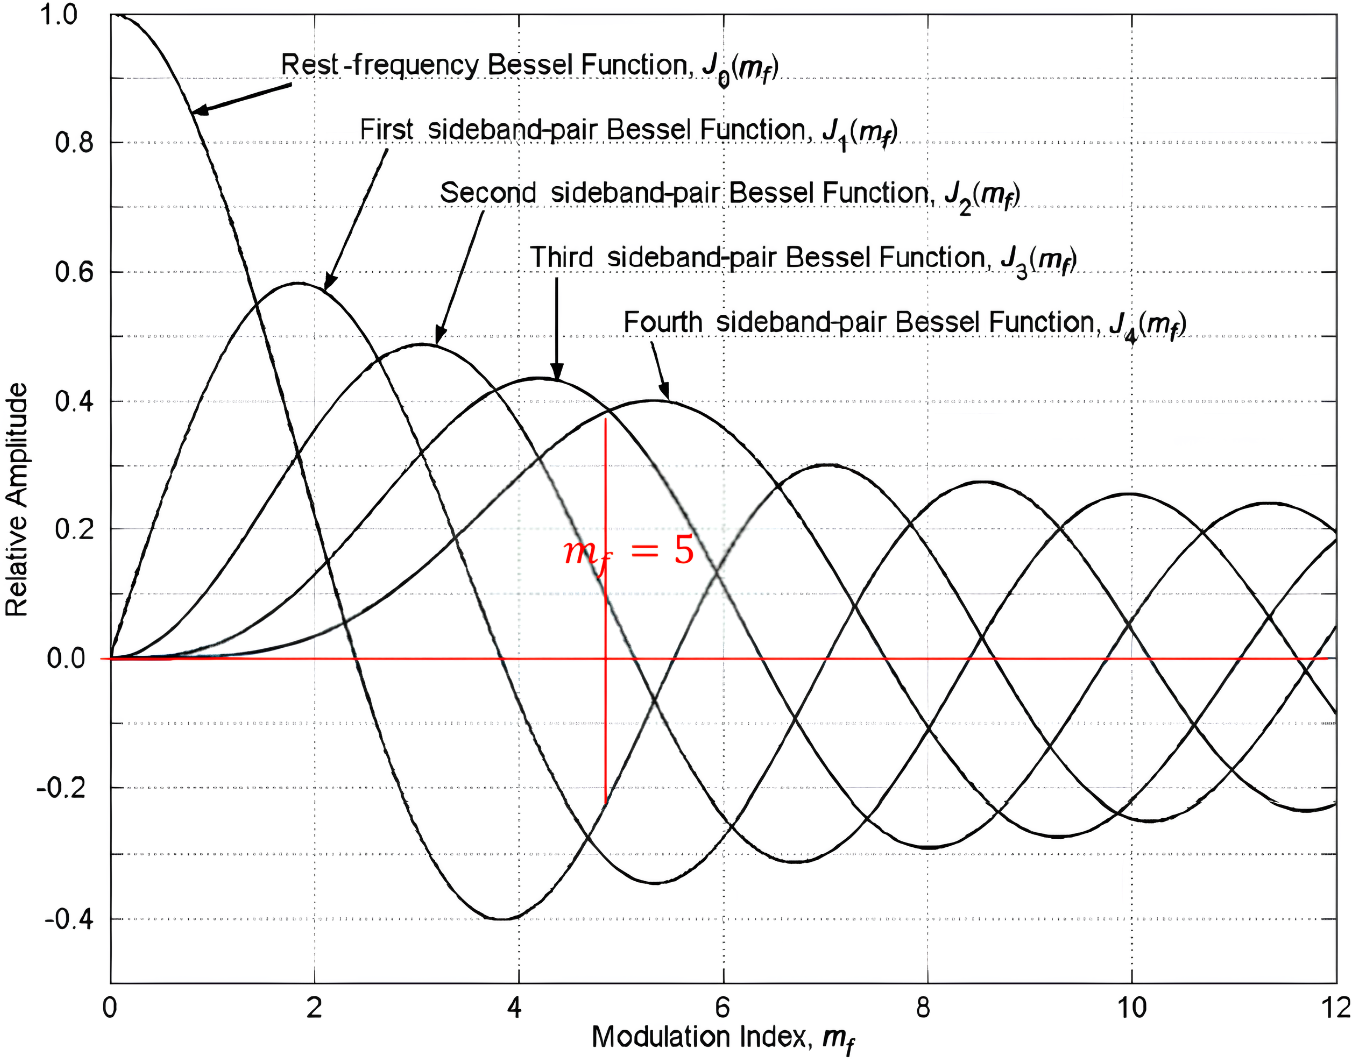
\includegraphics[width=0.625\textwidth]{imgs/bessel1.png}
\end{center}


\begin{center}
    \resizebox{0.75\textwidth}{!}{
        \begin{tikzpicture}

            % Axis
            \draw[->] (0,0) -- (12,0) node[right, font=\small] {Frequency};
            \draw[->] (0,0) -- (0,7.5) node[above, font=\small] {Amplitude};
        
        
            \foreach \x [count=\xi from 0] in {1.5,3,4.5,6,7.5,9,10.5} {
                \pgfmathsetmacro{\mu}{6}  % Median of the x values
                \pgfmathsetmacro{\sigma}{2}  % Standard deviation (you can adjust this value)
                \pgfmathsetmacro{\A}{6}  % Amplitude (scaling factor)
                
                \pgfmathsetmacro{\y}{\A * exp(-((\x - \mu)^2) / (2 * \sigma^2))}
                
                % Draw the line
                \draw (\x,0) -- (\x,{\y}) node[above] {};
            }

            % Frequency labels
            \node[below, font=\small] at (1.5,0) {$f_c - 3f_m$};
            \node[below, font=\small] at (3,0) {$f_c - 2f_m$};
            \node[below, font=\small] at (4.5,0) {$f_c - f_m$};
            \node[below, font=\small] at (6,0) {$f_c$};
            \node[below, font=\small] at (7.5,0) {$f_c + f_m$};
            \node[below, font=\small] at (9,0) {$f_c + 2f_m$};
            \node[below, font=\small] at (10.5,0) {$f_c + 3f_m$};
            
            % fm arrow
            \draw[<->, red] (6,0.75) -- node[above, font=\small] {\textcolor{red}{$f_m$}} (7.5,0.75);
            
        \end{tikzpicture}
    }
\end{center}

Ogni componente sinusoidale ha una frequenza che è un multiplo intero della frequenza di modulazione \( f_m \).
Queste componenti sono chiamate "sidebands", e la loro ampiezza è determinata dalle funzioni di Bessel \( J_n(m_f) \).
La frequenza della portante appare come il picco centrale nello spettro (per \( n = 0 \)), con la sua ampiezza modulata da \( J_0(m_f) \).

In generale, l'ampiezza delle funzioni di Bessel (e quindi delle bande laterali) diminuisce all'aumentare di \( |n| \), anche se questo decadimento non è necessariamente monotono.
Il pattern esatto dipende dal valore dell'indice di modulazione \( m_f \), un indice di modulazione più alto distribuisce più energia nelle bande laterali di ordine superiore, allargando la banda del segnale FM,
infatti si può vedere graficamente come più è l'indice di modulazione, più è grande il numero di funzioni di Bessel di cui devo tenere conto quando rappresento lo spettro del segnale FM.
Lo spettro è simmetrico rispetto alla frequenza della portante perché \( J_{-n}(m_f) = (-1)^n J_n(m_f) \). Quindi, per ogni componente di frequenza positiva, c'è una corrispondente componente di frequenza negativa con la stessa ampiezza ma potenzialmente fase diversa (a seconda che \( n \) sia dispari o pari).
La banda di Carson approssima la larghezza di banda del segnale FM a:
\[
    B_{FM} \approx 2(\Delta f + f_{m}) = 2(m_f + 1) f_{m}
\]
\[
    \Delta f \coloneqq \text{max} \{ | f_d(t) | \} = k_f \cdot \text{max} \{ | m(t) | \}
\]
% TODO: qual è la differenza tra % f_{max} e f_m e B?
Dove \( \Delta f \) è la deviazione massima della frequenza, \( f_{m} \) è la frequenza massima del segnale modulante e \( m_f \) è l'indice di modulazione.
Questa regola stima la banda in cui è concentrata la maggior parte dell'energia del segnale FM.
Ogni segnale modulato in frequenza ha un numero infinito di bande laterali e quindi una banda infinita. Ma la maggior parte dell'energia (98\% o più) è concentrata all'interno della banda definita dalla regola di Carson. Per la radio FM mono commerciale:
\begin{align*}
f_m &= 15 \text{ kHz (high quality audio)}, \\
\Delta f &= 75 \text{ kHz}, \\
m_f &= 5, \\
B_{FM} &\approx 180 \text{ kHz}.
\end{align*}

\paragraph*{Ricevitore FM}
Trascurando il rumore, il segnale ricevuto assume la forma:
\[
\hat{v}(t) = A_c e^{j2\pi k_f \int_{-\infty}^{t} m(\tau) d\tau}
\]
Che può quindi essere demodulato differenziando la fase di \( \hat{v}(t) \):
\[
\hat{m}(t) = \frac{1}{2\pi k_f} \frac{d}{dt} \angle \hat{v}(t)
\]


\begin{center}

    \begin{tikzpicture}[
            block/.style={rectangle, draw, minimum height=1cm, minimum width=1.5cm},
            node distance=1cm and 1cm,
            auto
        ]
        % Blocks
        \node[inner sep=0pt, minimum size=0pt] (source) {};
        \node[block, right=of source] (encoder) {$\angle$};
        \node[block, right=of encoder] (interp) {$\frac{d}{dt}$};

        % create a node which is above interp
        \node[above=of interp, inner sep=0pt, minimum size=0pt] (dummy1) {};
        \node[below=of interp, inner sep=0pt, minimum size=0pt] (dummy2) {};




        \node[draw, circle, right=1cm of interp] (m1) {\(\times\)};

        \draw[->] (interp) -- (m1);
        \node[below=of m1] (cos) {};
        \draw[->] (cos) -- (m1) node[midway, right] {$\frac{1}{2\pi k_f}$};


        \node[right=1cm of m1, inner sep=0pt, minimum size=0pt] (dummy3) {};


        \draw[->] (m1) -- (dummy3) node[midway, above] {$\hat{m}(t)$};



        %\draw[->] (interp) -- node[midway, above] {$x_c[n]$} (p1);

        \draw[->] (source) -- (encoder) node[midway,above] {$\tilde{v}(t)$};
        \draw[->] (encoder) -- (interp) node[midway,above] {};


    \end{tikzpicture}
\end{center}


Supponiamo che a causa della differenza tra trasmettitore e ricevitore ci sia adesso una frequenza $\Delta f$ (per esempio potrebbe essere anche solo 10 Hz)
\[
    v(t) = e^{j2\pi \Delta f t + j2 \pi k_f \int_{-\infty}^{t} m(\tau) d\tau}
\]

e quindi la fase sarà:
\[
    \angle v(t) = 2\pi \Delta f t + 2\pi k_f \int_{-\infty}^{t} m(\tau) d\tau
\]
da cui:
\[
    \frac{1}{2\pi k_f}  \frac{d}{dt} \angle v(t) = \frac{\Delta f}{k_f} + m(t)
\]

e da come possiamo notare, $\frac{\Delta f}{k_f}$ è solo una costante aggiunta al segnale. Come tale, sta sulla frequenza 0 che non può essere udita dall'orecchio umano. Quando la costante $\Delta f$ è grande, comunque, quando vogliamo prendere l'energia del segnale, parte del segnale potrebbe essere filtrata.% (TODO: Perché?).


\section*{Software Defined Radio (SDR)}
Le componenti di un sistema radio sono generalmente realizzate tramite dispositivi hardware analogici.
Le recenti innovazioni tecnologiche hanno permesso di implementare tali componenti direttamente in software.
All'interno di un ricevitore SDR il segnale in arrivo è convertito in formato digitale per essere processato.
La componente software permette una semplice riprogrammazione, in tal modo è possibile modificare l'elaborazione del segnale senza dover cambiare componenti fisiche del sistema.
La tecnica SDR deriva dal campo delle trasmissioni militari in cui è necessario equipaggiare i soldati con molte componenti radio per gestire le numerose comunicazioni da realizzare.
L'introduzione del SDR ha permesso di semplificare l'equipaggiamento, riducendo il numero di dispositivi necessari per supportare i protocolli radio militari.

Il campo in cui le tecniche SDR hanno portato innumerevoli vantaggi è quello della ricerca e sviluppo, perché il passaggio da design hardware a programmazione ha permesso di velocizzare i tempi di sviluppo di nuove tecnologie.

La chiave per lo sviluppo delle tecniche SDR è il miglioramento delle capacità di calcolo dei processori, perché sono in grado di applicare l'elaborazione precedentemente realizzata completamente in hardware specializzato.
Con il passaggio al software è possibile modificare l'elaborazione del segnale senza dover cambiare componenti fisiche del sistema, semplificando il processo di sviluppo e riducendo i costi, introducendo eventuali nuovi formati di modulazione, algoritmi e applicazioni.


\subsection*{Architettura RTL-SDR}
% TODO: quali sono le connessioni notevoli tra le varie componenti?
% includi immagine in pdf chiamata imgs/sdr.pdf
\begin{center}
   % include sdr.pdf image
    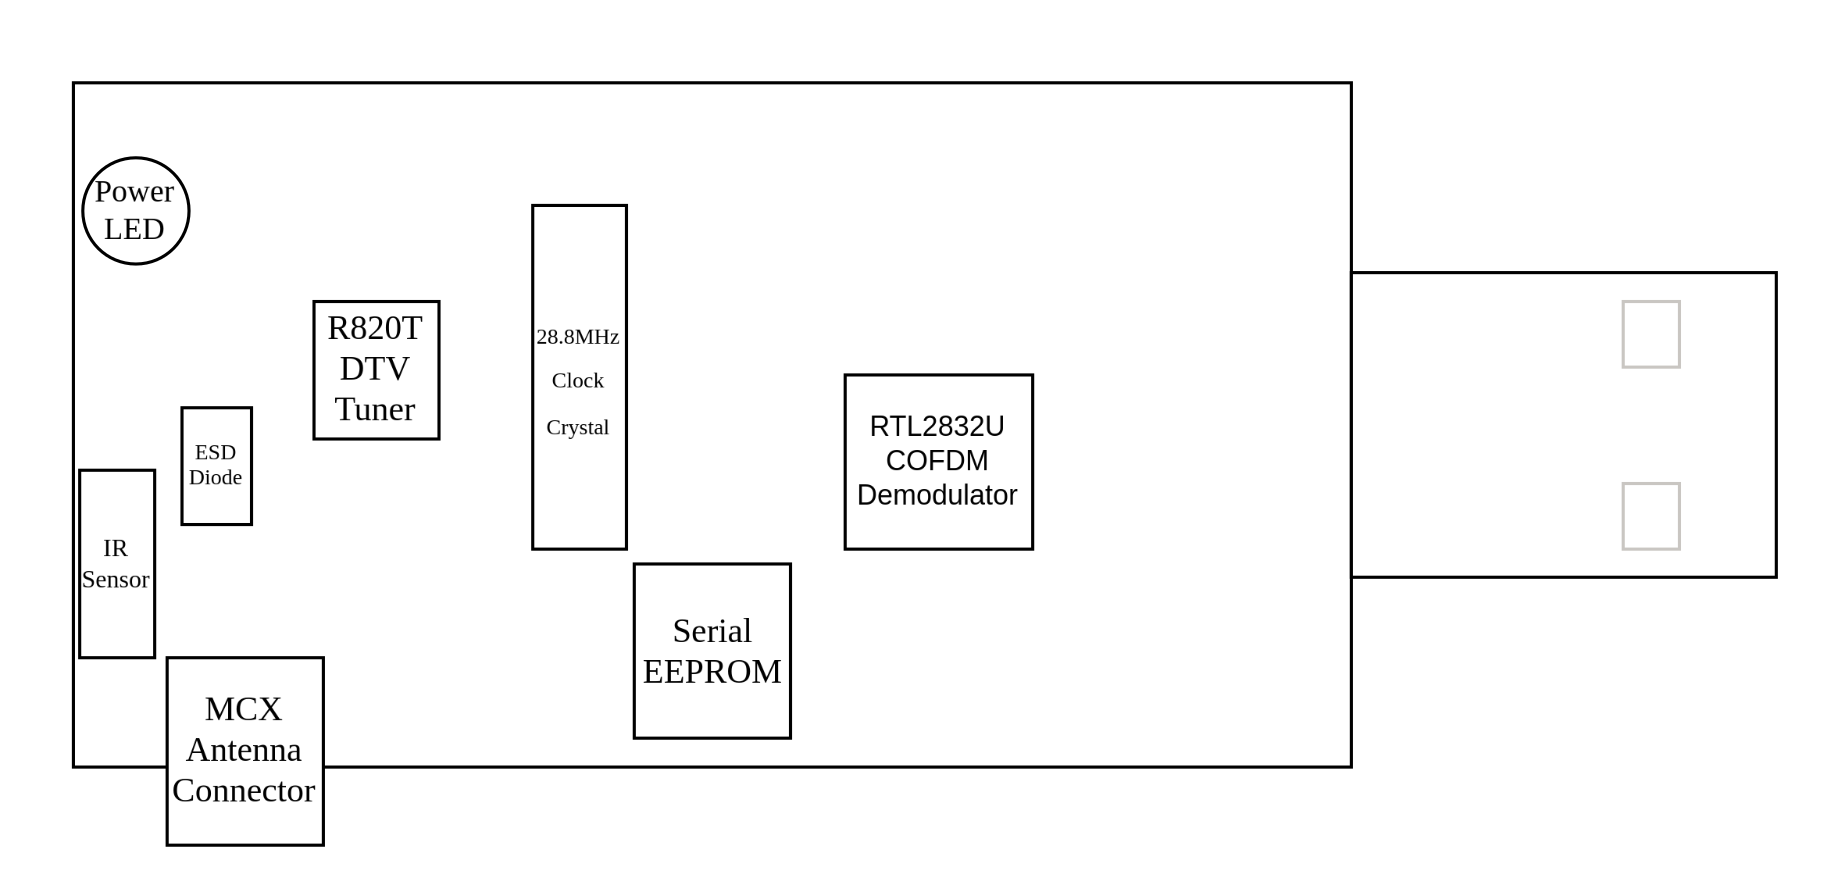
\includegraphics[width=0.8\textwidth]{imgs/sdr.png} 
\end{center}


Il RTL-SDR è un dispositivo inizialmente ideato per ricevere segnale TV su un PC, che è possibile hackerare settando un bit di debug nel driver, così che invierà tutti i campioni I/Q ricevuti dall'antenna. 
Il compito dell'RTL-SDR è prendere un chunk dello spettro del segnale ricevuto e convertirlo in banda base, che potrà poi essere processato dal software.
% Detailing the components of RTL-SDR

Le componenti principali sono:
\begin{itemize}
    \item \textbf{R820T DTV Tuner:} chip dedicato all'elaborazione del segnale in banda, responsabile della selezione della banda di frequenza del segnale desiderato dallo spettro RF.
    \item \textbf{28.8MHz Clock Crystal:} fornisce una frequenza di riferimento stabile per il tuner e il demodulatore, determina la banda massima che può essere ottenuta dai campioni I/Q.
    \item \textbf{RTL2832U COFDM Demodulator:} chip utilizzato per la conversione analogico-digitale, sebbene il nome "demodulator" possa essere fuorviante in questa fase non avviene nessuna demodulazione del segnale.
    \item \textbf{MCX Antenna Connector:} permette la connessione di diversi tipi di antenne.
    \item \textbf{Serial EEPROM:} memorizza i dati di configurazione del dispositivo USB.
    \item \textbf{USB 2.0 Interface:} permette la connessione con i computer per l'elaborazione successiva.
    \item Componenti aggiuntive come un \textbf{LED di alimentazione}, un \textbf{diodo ESD} e un \textbf{sensore IR} per l'interfacciamento con l'utente e la protezione del dispositivo.
\end{itemize}
% insert a piacture.png

Il dispositivo implementa un ricevitore super heterodyne, in cui il segnale in banda è prima trasformato in media frequenza (IF) e dopo alcune trasformazioni in banda base.
Questa doppia trasformazione è necessaria per ottimizzare l'amplificazione del segnale, più semplice a media frequenza rispetto al segnale in banda base.

\begin{center}
    \begin{tikzpicture}[
        block/.style={rectangle, draw, minimum height=2em, minimum width=3em},
        line/.style={draw, -Latex}
    ]
        \node[block, align=center] (rfFrontEnd) {Flexible RF \\ Front End};
        \node[block, right=0.5cm of rfFrontEnd, align=center] (adConverter) {A/D Converter};
        \node[block, right=0.5cm of adConverter, align=center] (demod) {Demodulation \\ to Bband};
        \node[block, right=0.5cm of demod, align=center] (decimation) {Decimation \\ Filtering};
        \node[block, right=0.5cm of decimation, align=center] (carrierSync) {Carrier \& Timing \\ Synchronisation};
        \node[block, right=0.5cm of carrierSync, align=center] (baseband) {Baseband \\ Processing};
        \node[inner sep=0pt, outer sep=0pt, above left=0.25cm and 0.05cm of rfFrontEnd] (antenna) {
\includegraphics[width=1cm]{imgs/antenna.pdf}};
        
        \draw[line] (rfFrontEnd) -- (adConverter);
        \draw[line] (adConverter) -- (demod);
        \draw[line] (demod) -- (decimation);
        \draw[line] (decimation) -- (carrierSync);
        \draw[line] (carrierSync) -- (baseband);
        \draw (rfFrontEnd.west) -- ++(-0.5, 0) -- ++(0,0.5);
        
        \node[draw, dashed, fit=(rfFrontEnd) (adConverter) (demod) (decimation), inner sep=0.2cm, label=above:RTL-SDR Hardware] (hardware) {};
        \node[draw, dashed, fit=(carrierSync) (baseband), inner sep=0.2cm, label=above:MATLAB / Simulink design (running on computer)] (software) {};
        
        \node[align=left, below=0.5cm of hardware.south] (freqRange) {Range: \\ 25MHz -- 1.75GHz};
        \node[align=left, below=0.5cm of software.south] (samplingFreq) {Sampling frequency (\(f_s\)): \\ up to around 2.8MHz};
    
        \node[inner sep=0pt, outer sep=0pt, right=0.5cm of baseband] (output) {
\includegraphics[width=1cm]{imgs/notes.pdf}};
        \draw[line] (baseband) -- (output);
    \end{tikzpicture}
\end{center}
% Explanation of the SDR block diagram for FM reception
The block diagram for an FM receiver using RTL-SDR hardware typically involves the following processing stages:
\begin{enumerate}
    \item \textbf{RF Antenna:} Captures the FM signal from the air.
    \item \textbf{Flexible RF Front End:} Filters and amplifies the RF signal from the antenna.
    \item \textbf{Analogue to Digital Converter (ADC):} Converts the analog RF signal to a digital format.
    \item \textbf{Demodulation to IQ Band:} The digital signal is demodulated into I (In-phase) and Q (Quadrature) components.
    \item \textbf{Decimation Filtering:} Reduces the sampling rate and noise, retaining the signal of interest.
    \item \textbf{Carrier \& Timing Synchronization:} Synchronizes the received signal with the local reference for accurate demodulation.
    \item \textbf{Baseband Processing:} This may involve MATLAB/Simulink running on a computer to process the demodulated signal.
    \item \textbf{Baseband Output:} The final audio signal is output, ready for listening.
\end{enumerate}
The signal processing range for this system is from 25MHz to 1.75GHz with a sampling frequency (IF) up to around 2.8MHz.
\begin{center}
    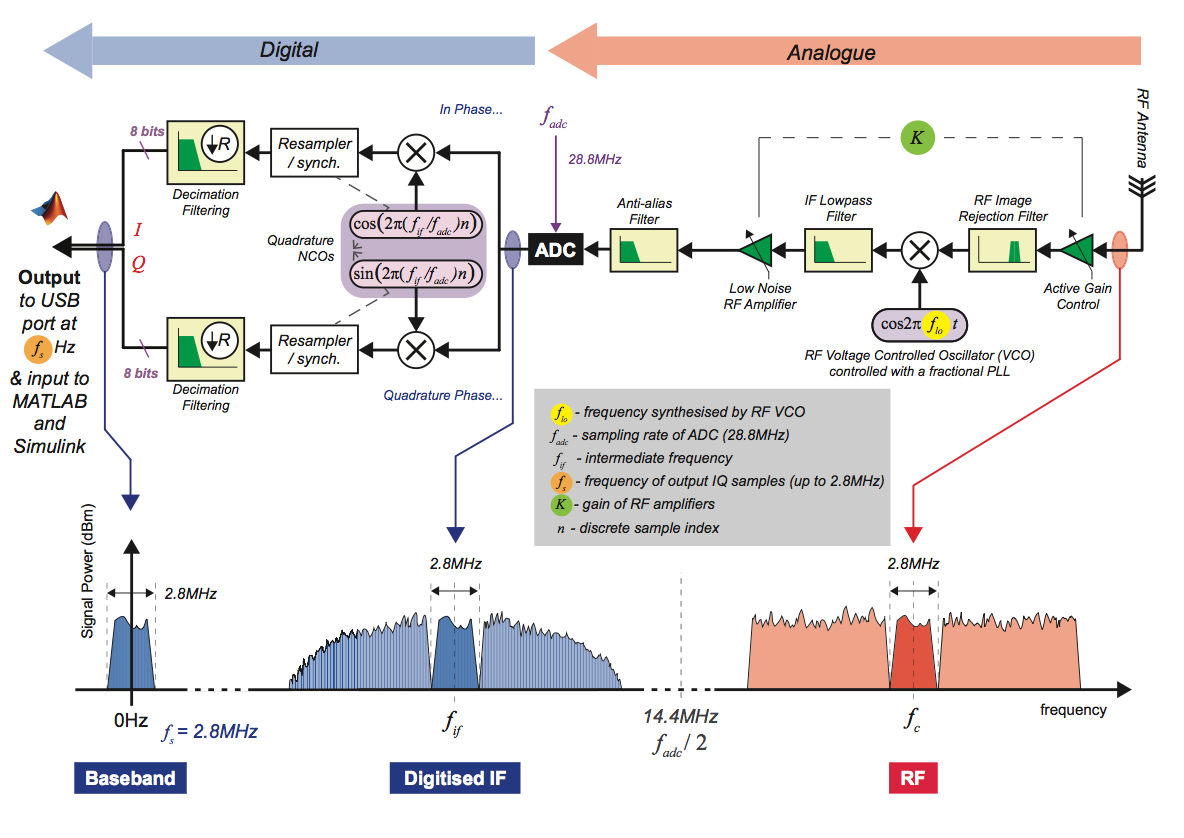
\includegraphics[width=0.9\textwidth]{imgs/rtl-sdr.png}
\end{center}

\section*{RTL-SDR Receiving Steps}




\begin{center}

    \begin{tikzpicture}[
            block/.style={rectangle, draw, minimum height=1cm, minimum width=1.5cm},
            node distance=1cm and 1cm,
            auto
        ]

        \tikzstyle{tri} = [draw, isosceles triangle, isosceles triangle apex angle=60, shape border rotate=360, minimum height=2em]
        % Blocks
        \node[inner sep=0pt, minimum size=0pt] (source) {};


        \node[tri, right=of source] (encoder) {};
        \node[block, right=of encoder] (interp) {BPF};

        % create a node which is above interp
        \node[above=of interp, inner sep=0pt, minimum size=0pt] (dummy1) {};
        \node[below=of interp, inner sep=0pt, minimum size=0pt] (dummy2) {};

        \node[draw, circle, right=1cm of interp] (m1) {\(\times\)};

        \draw[->] (interp) -- (m1);
        \node[below=of m1] (cos) {};
        \draw[->] (cos) -- (m1) node[midway, right] {$\cos(2\pi(f_{LO} - f_{IF})t)$};


        %\node[right=1cm of m1, inner sep=0pt, minimum size=0pt] (dummy3) {};
        \node[tri, right=of m1] (dummy3) {};

        \draw[->] (m1) -- (dummy3) node[midway, above] {};
        \node[right=1cm of dummy3, inner sep=0pt, minimum size=0pt] (dummy4) {};
        \draw[->] (dummy3) -- (dummy4) node[midway, above] {};

        %\draw[->] (interp) -- node[midway, above] {$x_c[n]$} (p1);

        \draw[->] (source) -- (encoder) node[midway,above] {};
        \draw[->] (encoder) -- (interp) node[midway,above] {};


    \end{tikzpicture}
\end{center}



Il processo di eterodinazione è essenziale per convertire le frequenze radio più alte in frequenze più basse, più facili da amplificare e processare.
Nel disegno, $f_{LO}$ rappresenta la frequenza dell'oscillatore locale, mentre $f_{IF}$ (ovvero 3.57 MHz) è la frequenza intermedia a cui il segnale viene convertito, in cui avvengono anche una serie di filtraggi e amplificazioni.
Successivamente avverrà anche la conversione analogico-digitale con campionamento a 28.8 MS/s, dunque rispettamendo abbondantemente il teorema di Nyquist ($f_s > 2 (f + B)$) fino a una banda di $14.4$ MHz, in quanto \( 28.8 \si{MS/s} > 2 \times (3.57 \si{MHz} + B) \).% (TODO: ultima affermazione da controllare).

Campionando $\cos(2\pi f_{IF} t)$ si ottiene:
\[
    \cos(2\pi f_{IF} n T_s) = \cos(2\pi \frac{f_{IF}}{f_{ADC}} n)
\]

La frequenza di campionamento determina la massima banda estraibile dal segnale, ovvero 2.8 MHz

\begin{center}
    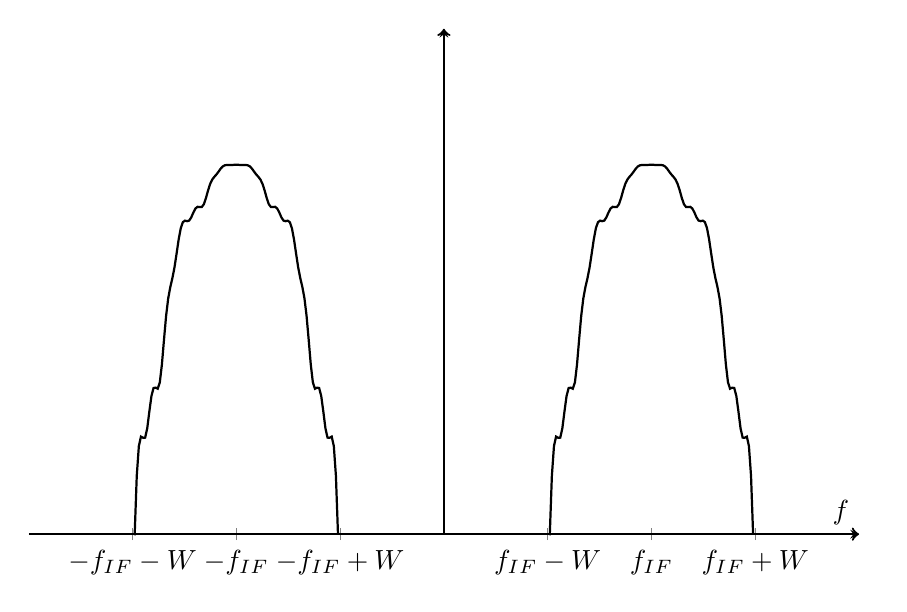
\begin{tikzpicture}
        \begin{axis}[
            axis lines=middle,
            width=\textwidth,
            height=8cm,
            xlabel={$f$},
            ylabel={},
            xtick={-3,-2,-1,0,1,2,3},
            xticklabels={$-f_{IF}-W$, $-f_{IF}$, $-f_{IF}+W$, $0$, $f_{IF}-W$, $f_{IF}$, $f_{IF}+W$},
            ytick=\empty,
            xmin=-4,
            xmax=4,
            ymin=0,
            ymax=1,
            clip=false
        ]

        \pgfmathsetmacro{\fIF}{2}
        \pgfmathsetmacro{\W}{1}

        \addplot[domain=-\fIF-\W:-\fIF+\W, samples=100, black, thick] 
            ({x}, {((sqrt(-15129*(x+\fIF)^2 + 1968*(x+\fIF)*sin(deg(15*(x+\fIF)))^3 - 64*sin(deg(15*(x+\fIF)))^6 + 14400))/(120))} - 0.269 );
        \addplot[domain=\fIF-\W:\fIF+\W, samples=100, black, thick] 
            ({x}, {((sqrt(-15129*(x-\fIF)^2 + 1968*(x-\fIF)*sin(deg(15*(x-\fIF)))^3 - 64*sin(deg(15*(x-\fIF)))^6 + 14400))/(120))} - 0.269 );

        \draw[->,thick] (axis cs:-4,0) -- (axis cs:4,0) node[right] {};
        \draw[->,thick] (axis cs:0,0) -- (axis cs:0,1);

        \end{axis}
    \end{tikzpicture}
\end{center}
% TODO: cos'è il mixer?
Nella figura è rappresentato il segnale in uscita dal mixer, con frequenza intermedia $f_{IF} = 3.57$ MHz e banda $W = 1.4$ MHz.

Ogni sample è composto da 8 bit. I sample del segnale campionato seguono un percorso parallelo per estrarre la commponente in fase e in quadratura. Entrambi i rami effettuano la conversione da media a frequenza a banda base.
Avvengono una serie di operazioni che permettono di estrarre la banda che sarà rappresentata dai sample I/Q in uscita da ques'ultima fase tramite interfaccia USB.
La fase di decimation permette di adattare il campionamente  del segnale al valore richiesto dell'utente. Il rate massimo è circa 2.8 MS/s.
Lo spettro di frequenza in grado di essere captato dal dispositivo risulta approssimativamente (TODO).
Bisogna comunque tenere in considerazione che la banda limitata a 2.8 MHz non permette di estrarre informazioni di modulazioni che richiedano una banda superiore, ad esempio il Wi-Fi.


\paragraph*{Ricezione radio FM}
\begin{center}
    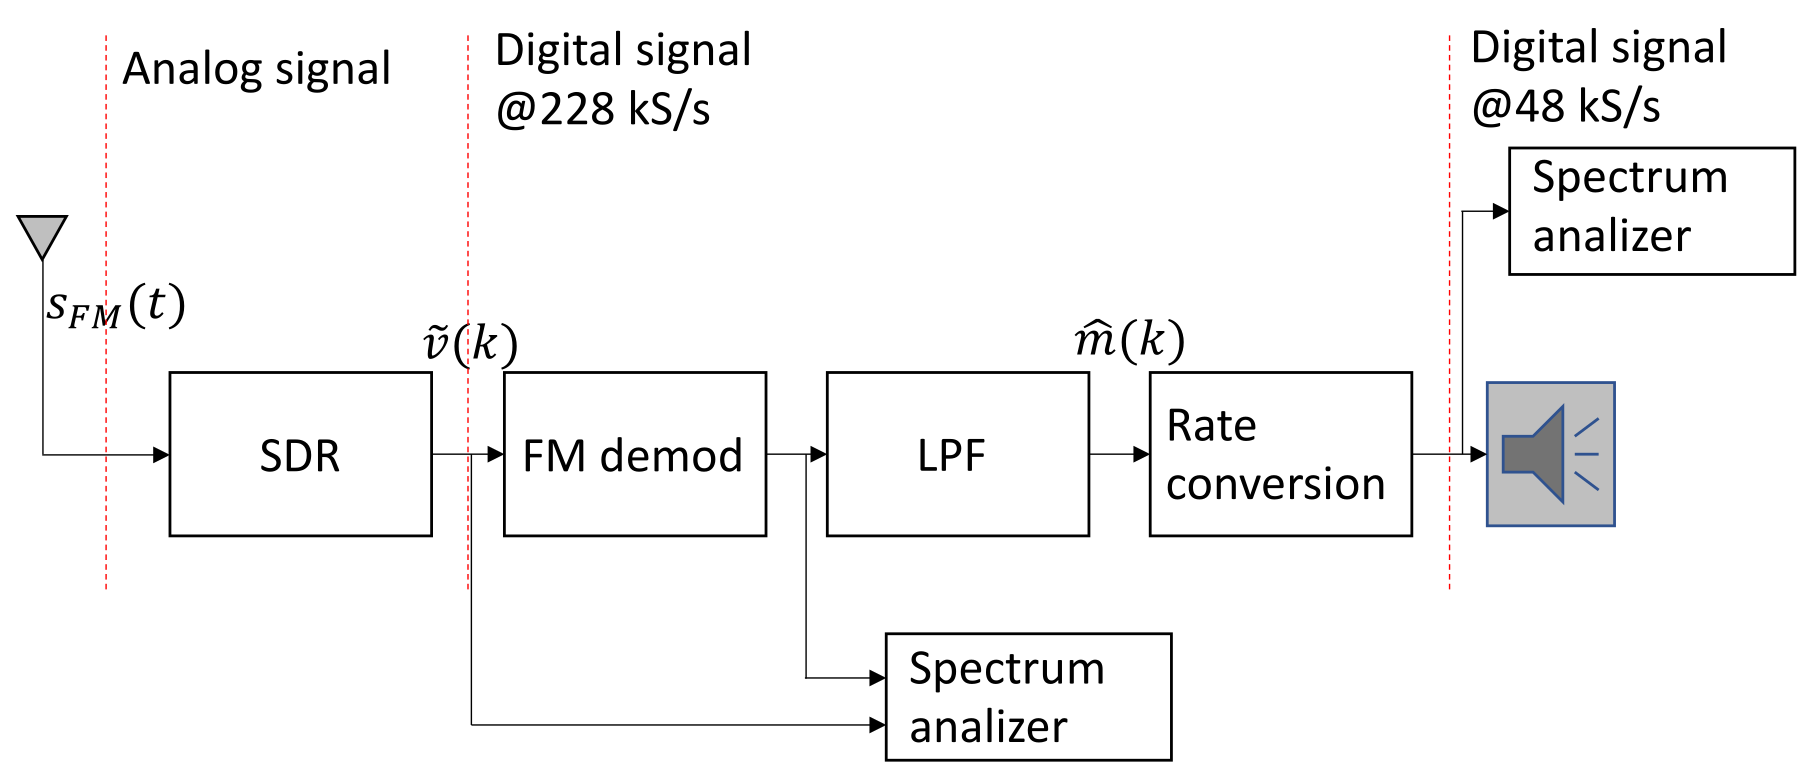
\includegraphics[width=0.75\textwidth]{imgs/fm_receiver_impl.jpg}
\end{center}
I simboli I/Q digitali ricevuti dal SDR richiedono una demodulazione per essere convertiti nell'informazione trasmessa. In particolare per la radio FM si considera
\[
    m(t) = L(t) + R(t)
\]
segnale FM mono, normalizzato ad 1, ovvero $\max{m(t)} = 1$ e quindi $\Delta f = k_f$.


L'inviluppo complesso del segnale ricevuto assume la forma:

\[
    \tilde{v}(t) = A_c e^{j2\pi k_f \int_{-\infty}^{t} m(\tau) d\tau}
\]

Campionando in $T_s$ si ottiene:
\[
    \tilde{v}(kT_s) = \tilde{v}[k] = A_c e^{j2\pi k_f \int_{-\infty}^{kT_s} m(\tau) d\tau}
\]

che può essere approssimato in
\[
    \tilde{v}[k] \approx A_c e^{j2\pi k_f \sum_{\ell = -\infty}^{k} m[\ell] \ T_s}
\]

moltiplicando per il coniugato del campione precedente si ottiene
\[
  \tilde{v}[k] \ \tilde{v}^*[k-1] \approx A_c^2 e^{j2\pi k_f \sum_{\ell = -\infty}^{k} m[\ell] \ T_s} e^{-j2\pi k_f \sum_{\ell = -\infty}^{k-1} m[\ell] \ T_s} = A_c^2 e^{j2\pi k_f m[k] \ T_s}
\]


da cui:
\[
    \tilde{m}[k] = \frac{1}{2\pi k_f T_s} \angle \left( \tilde{v}[k] \ \tilde{v}^*[k-1] \right)
\]

